
\documentclass[template=tabling,81pt,headonall]{azmoon}
\usepackage{xepersian}
\usepackage{amsfonts}
\usepackage{graphicx}
\graphicspath{ {./images/} }
\settextfont{Yas}
\setdigitfont{A Iranian Sans}

\printanswers
    \teacher{محمد صالح علی اکبری}
    \teachertitle{دبیر}
    \city{گناباد}
    \schooltitle{متوسطه دوره دوم}
    \school{شاهد امام (ره)}
    \grade{هفتم}
    \branch{-}
    \topic{ریاضی}
    \examdate{شهریور 1402}
    \answertime{120 دقیقه}
    \begin{document}
	\begin{questions}
		\nointerlineskip%
		\vskip-\baselineskip
		\question{%
عبارت‌های زیر راحساب کنید.
    \begin{LTR}
        \begin{parts}[1]\part{$-73 + (-82) \times 2 + 7 -43 \times (-3) = $}
‌\\\part{$\dfrac{\dfrac{32}{-2}}{\dfrac{-30}{6}}$}
\end{parts}
\end{LTR}
        ‌
\\
    }\question{%
در تصویر دهم چند چوب کبریت وجود دارد؟ \\ در شکل n ام چند چوب کبریت وجود دارد؟ \\ 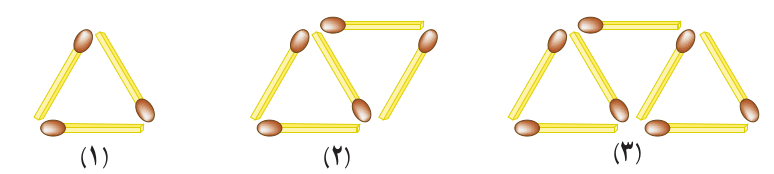
\includegraphics[scale = 0.3]{donbale_choob_kebriti}‌
\\‌
\\}\question{%
معادله‌های زیر را حل کنید:
    \begin{LTR}
        \begin{parts}[1]\part{$8x - 4 = 27$}
‌\\‌\\\part{$3x = 6x - 7$}
\end{parts}
\end{LTR}
        ‌
\\‌
\\‌
\\
    }\question{%
عبارت‌های زیر را در صورت امکان \underline{به کمک توان} ساده کنید.
    \begin{LTR}
        \begin{parts}[1]\part{$3+3+3$}
\part{$2 \times 2 \times 2 \times 2 =$}
\end{parts}
\end{LTR}
        
    }\question{%
تساوی‌های زیر را کامل کنید.(به شکل عبارت توان دار بنویسید.)
    \begin{LTR}
        \begin{parts}[1]\part{$(x + y) ( x + y ) = $}
‌\\\part{$\dfrac{y \times y \times y \times y \times y}{x \times x \times x} =$}
\end{parts}
\end{LTR}
        ‌
\\
    }\question{%
با رعایت اولویت‌های محاسباتی عبارت‌های زیر را حساب کنید.
    \begin{LTR}
        \begin{parts}[1]\part{$2 \times 3^{2} - (2^{2} + 2)$}
‌\\\part{$\dfrac{10 \div (8 - 6)+9 \times 4}{2^{5}+3^{5}}$}
\end{parts}
\end{LTR}
        
    }\question{%
حاصل عبارت‌های زیر را حساب کنید.
    \begin{LTR}
        \begin{parts}[2]\part{$\sqrt{\dfrac{9}{25}}$}
\part{$-\sqrt{49}$}
\end{parts}
\end{LTR}
        ‌
\\
    }\question{%
هر یک از اعداد زیر بین کدام دو عدد صحیح متوالی قرار دارد؟ توضیح دهید.
    \begin{LTR}
        \begin{parts}[1]\part{$\sqrt{7}$}
\part{$\sqrt{60}$}
\part{$-\sqrt{42}$}
\end{parts}
\end{LTR}
        
    }\question{%
بردار $\begin{bmatrix} -3 \\ 2 \end{bmatrix}$ را در محور مختصات زیر رسم کنید که ابتدای بردار نقطه $\begin{bmatrix} 3 \\ -2 \end{bmatrix}$ باشد.
\\ مختصات نقطه انتهای آن را بنویسید. \\
باتوجه به شکل مختصات نقطه‌ها و بردارهای زیر را بنویسید. \\
$A = \begin{bmatrix} \ \ \ \\  \end{bmatrix}$ \ $B = \begin{bmatrix} \ \ \ \\  \end{bmatrix}$ \ $\overrightarrow{AB} = \begin{bmatrix} \ \ \ \\  \end{bmatrix}$ \ $D = \begin{bmatrix} \ \ \ \\  \end{bmatrix}$ \ $C = \begin{bmatrix} \ \ \ \\  \end{bmatrix}$ \ $\overrightarrow{CD} = \begin{bmatrix} \ \ \ \\  \end{bmatrix}$ \
\\
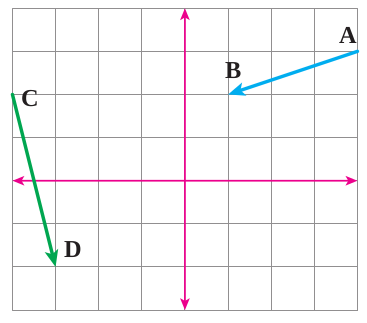
\includegraphics[scale = 0.3]{mokhtasat_haftom}}\question{%
مختصات مورد نظر (مقدار x و y ) را بدست بیاورید. \\
    \begin{LTR}
        \begin{parts}[1]\part{ $\begin{bmatrix} x \\ y \end{bmatrix} + \begin{bmatrix} -1 \\ 2 \end{bmatrix} = \begin{bmatrix} 2 \\ -1 \end{bmatrix}$}
‌\\‌\\\part{$\begin{bmatrix} -4 \\ 3 \end{bmatrix} + \begin{bmatrix} 2 \\ -1 \end{bmatrix} = \begin{bmatrix} x \\ -y \end{bmatrix}$}
\end{parts}
\end{LTR}
        ‌
\\‌
\\
    }\question{%
شمارنده‌های اعداد زیر را جلوی آن‌ها بنویسید.
    \begin{parts}[1]\part{شمارنده‌های 12}
\part{شمارنده‌های 18}
\part{شمارنده‌های 25}
\part{شمارنده‌های 53}
\end{parts}

    }\question{%
با تجزیه کردن (نوشتتن عدد به صورت ضرب عامل‌های اول) عددهای صورت و مخرج، کسرها را تا حد امکان ساده کنید. در واقع شمارنده‌های مشترک صورت و مخرج را ساده کنید.
    \begin{LTR}
        \begin{parts}[2]\part{$\dfrac{126}{39}$}
\part{$\dfrac{50}{20}$}
‌\\\part{$\dfrac{81}{32}$}
\part{$\dfrac{42}{21}$}
\end{parts}
\end{LTR}
        ‌
\\
    }\question{%
ب.م.م. و ک.م.م. های زیر را حساب کنید.
    \begin{LTR}
        \begin{parts}[3]\part{$[12 , 18]$}
\part{$[25 , 35]$}
\part{$(35 , 28)$}
‌\\‌\\‌\\\part{$(7 , 3 , 5)$}
\part{$[100 , 25 , 4]$}
\part{$(32 , 28)$}
‌\\‌\\‌\\\part{$(70 , 6)$}
\part{$[30 , 7 , 6]$}
\part{$(30 , 7 , 6)$}
\end{parts}
\end{LTR}
        ‌
\\‌
\\
    }\end{questions}
    \end{document}
    